\documentclass[a4paper]{article}
\setlength{\topmargin}{-1.0in}
\setlength{\oddsidemargin}{-0.2in}
\setlength{\evensidemargin}{0in}
\setlength{\textheight}{10.5in}
\setlength{\textwidth}{6.5in}
\usepackage{enumitem}
\usepackage{amsmath}
\usepackage{hyperref}
\usepackage{amssymb}
\usepackage[dvipsnames] {xcolor}
\usepackage{mathpartir}
\usepackage{algorithm}
\usepackage{algpseudocode}
\usepackage{csquotes}
\usepackage{tikz}
\usetikzlibrary{positioning,arrows.meta}

\hbadness=10000

\hypersetup{
    colorlinks=true,
    linkcolor=blue,
    filecolor=magenta,      
    urlcolor=cyan,
    pdftitle={Assignment 1},
    pdfpagemode=FullScreen,
    }
\def\endproofmark{$\Box$}
\newenvironment{proof}{\par{\bf Proof}:}{\endproofmark\smallskip}
\begin{document}
\begin{center}
{\large \bf \color{red}  Department of Computer Science} \\
{\large \bf \color{red}  Ashoka University} \\

\vspace{0.1in}

{\large \bf \color{blue} Reinforcement Learning} \\

\vspace{0.05in}

    { \bf \color{YellowOrange} Assignment 1}
\end{center}
\medskip

{\textbf{Collaborators:} None} \hfill {\textbf{Name: Rushil Gupta} }

\bigskip
\hrule


% Begin your assignment here %
\section*{Problem 1}
\subsection*{Part (a)}

We want to minimize the number of steps the agent takes. So, setting $r_s = -1$ would mean that we are penalizing the agent for being at any non-terminal square. Moreover, since $r_r = -5$ and $r_g = 5$, the agent would be incentivized to reach the green square and avoid the red square.\\

\noindent Now, to find the optimal value for each square, we use:

\[
V(s) = r_s + \max_{a} \left[V(s') \right]
\]

\noindent We know $V(12) = 5$ and $V(5) = -5$. We can now calculate the value of each square by backtracking from the terminal states. After inspection, the value of each square boils down to $5 - n$, where $n$ is the minimum number of steps needed to reach the green square. So:
\begin{align*}
V(1) &= 0 \\
V(2) &= 1 \\
V(3) &= 2 \\
V(4) &= 3 \\
V(6) &= 2 \\
V(7) &= 3 \\
V(8) &= 4 \\
V(9) &= 2 \\
V(10) &= 3 \\
V(11) &= 4 \\
V(13) &= 1 \\
V(14) &= 0 \\
V(15) &= -1 \\
V(16) &= -2 \\
\end{align*}


\subsection*{Part (b)}
Given a policy $\pi$ and its associated value function $V^{\pi}_{old}$, we want to see how $V^{\pi}_{old}$ changes when we add $c$ to each reward. Recall that $V^{\pi}_{old}$ is given by:

\[
V^{\pi}_{old}(s) = r_s + \gamma \cdot V^{\pi}_{old}(\pi(s))
\]

\noindent where $\pi(s)$ is the new state that we reach after taking the action specified by $\pi$ (since we know each action has a deterministic outcome). Now, if we add $c$ to each reward, we get $V^{\pi}$ as:

\begin{align*}
V^{\pi}(s) &= (r_s + c) + \gamma \cdot V^{\pi}(\pi(s)) \\
V^{\pi}(s) &= (r_s + c) + \gamma \cdot \left(r_{\pi(s)} + c + \gamma \cdot V^{\pi}(\pi(\pi(s))) \right) \\
\vdots \\
V^{\pi}(s) &= r_s + \gamma \cdot V^{\pi}_{old}(\pi(s)) + c \cdot \left(1 + \gamma + \gamma^2 + \ldots \right) \\
V^{\pi}(s) &= V^{\pi}_{old}(s) + c \cdot \left(\frac{1}{1 - \gamma} \right)
\end{align*}

\noindent So, $V^{\pi}$ increases by a constant factor of $\frac{c}{1 - \gamma}$ when we add $c$ to each reward.


\subsection*{Part (c)}
We want to find a new value for $r_s$ such that the optimal policy will have at least one unshaded square that will take us to the red square. So, we want do this by looking at the value of 2 policies for each unshaded square, where the first policy is to go to the green square and the second policy is to go to the red square. We can then compare the values of these 2 policies and set $r_s$ such that the value of the policy that goes to the red square is greater than the value of the policy that goes to the green square for at least one unshaded square.\\

\noindent Let $s$ be some unshaded square, and let $d_{s,g}$, $d_{s,r}$ be the number of steps needed to reach the green and red squares respectively from $s$. Let $V^{g}$ and $V^{r}$ be the values of the policies that go to the green and red squares respectively. Then, we have:

\begin{align*}
V^{g}(s) &= r_g + d_{s,g} \cdot r_s = 5 + d_{s,g} \cdot r_s \\
V^{r}(s) &= r_r + d_{s,r} \cdot r_s = -5 + d_{s,r} \cdot r_s
\end{align*}

\noindent So, we need:
\begin{align*}
    5 + d_{s,g} \cdot r_s &< -5 + d_{s,r} \cdot r_s \\
    10 &< \left( d_{s,r} - d_{s,g} \right) \cdot r_s \\
\end{align*}

\noindent For simplicity, we will choose a square near the red square, say $s = 6$. We have $d_{6,g} = 3$ and $d_{6,r} = 1$. So, we need $10 < (1 - 3) \cdot r_s$. So, we can set $r_s = -6$ to satisfy this condition.\\

\noindent Now, we can calculate the value of both policies on square 6:
\begin{align*}
V^{g}(6) &= 5 + 3 \cdot -6 = -13 \\
V^{r}(6) &= -5 + 1 \cdot -6 = -11
\end{align*}

\noindent So, we know that by setting $r_s = -6$, the optimal policy will have at least one unshaded square that will take us to the red square.


\newpage
\section*{Problem 2}
\section*{Part (a)}
This problem is a shortest stochastic path problem. At each state, we have 2 actions, and a cost associated with each action. We want to find the shortest path from the start state (low) to the goal state (top). Here is the MDP:\\

\vspace{5mm}
\begin{tikzpicture}[node distance=1.8cm, auto, thick,
    state/.style={circle, draw=black, fill=white!5, very thick, minimum size=13mm},
    action/.style={rectangle, draw=red!60, fill=red!5, very thick, minimum size=10mm}]
  
    % Define state nodes
    \node[state] (Low) {Low};
    \node[state, right=of Low] (Medium) {Medium};
    \node[state, right=of Medium] (High) {High};
    \node[state, right=of High] (Top) {Top};
    \node[action, right=of Top] (Terminal) {Terminal};
  
    % Define action nodes
    \node[action, above=of Low] (Slow1) {Slow};
    \node[action, below=of Low] (Rapid1) {Rapid};
    \node[action, above=of Medium] (Slow2) {Slow};
    \node[action, below=of Medium] (Rapid2) {Rapid};
    \node[action, above=of High] (Slow3) {Slow};
    \node[action, below=of High] (Rapid3) {Rapid};
  
    % Arrows from states to actions (costs)
    \draw[->, bend left=30] (Low) to node [right] {\scriptsize $c=1$} (Slow1);
    \draw[->, bend right=30] (Low) to node [right] {\scriptsize $c=2$} (Rapid1);
    \draw[->, bend left=30] (Medium) to node [right] {\scriptsize $c=1$} (Slow2);
    \draw[->, bend right=30] (Medium) to node [right] {\scriptsize $c=2$} (Rapid2);
    \draw[->, bend left=30] (High) to node [right] {\scriptsize $c=1$} (Slow3);
    \draw[->, bend right=30] (High) to node [right] {\scriptsize $c=2$} (Rapid3);
    \draw[->, bend left=30] (Top) to node [above] {\scriptsize $c=0$} (Terminal);
  
    % Transitions from actions to next states (probabilities)
    \draw[->,bend left=20] (Slow1) to node [above,yshift=7pt] {\scriptsize$p=0.3$} (Medium);
    \draw[->, bend left=30] (Slow1) to node [right] {\scriptsize$p=0.7$} (Low);
    \draw[->, bend right=20] (Rapid1) to node [below,yshift=-7pt] {\scriptsize$p=0.5$} (Medium);
    \draw[->, bend right=30] (Rapid1) to node [right] {\scriptsize$p=0.5$} (Low);

    \draw[->, bend left=20] (Slow2) to node [above,yshift=7pt] {\scriptsize$p=0.3$} (High);
    \draw[->, bend left=30] (Slow2) to node [right] {\scriptsize$p=0.7$} (Medium);
    \draw[->, bend right=20] (Rapid2) to node [below,yshift=-7pt] {\scriptsize$p=0.5$} (High);
    \draw[->, bend right=30] (Rapid2) to node [right] {\scriptsize$p=0.5$} (Medium);

    \draw[->, bend left=20] (Slow3) to node [above,yshift=7pt] {\scriptsize$p=0.3$} (Top);
    \draw[->, bend left=30] (Slow3) to node [right] {\scriptsize$p=0.7$} (High);
    \draw[->, bend right=20] (Rapid3) to node [below,yshift=-7pt] {\scriptsize$p=0.5$} (Top);
    \draw[->, bend right=30] (Rapid3) to node [right] {\scriptsize$p=0.5$} (High);

    \draw[->, bend left=20] (Terminal) to node [below] {\scriptsize$p=1$} (Top);
\end{tikzpicture}

\subsection*{Part (b)}
This is done in the jupyter notebook.

\subsection*{Part (c)}
The optimal policiy suggests that we spin slowly when we are at the low and top states, and spin rapidly when we are at the medium and high states. Now, the first observation is once we reach the top state, we terminate immediately. So, the policy at this state can be ignored.\\

\noindent Now, let's look at the policy at the low state. The policy suggests that we spin slowly. On any other state, we spin rapidly. This is because on other states, if we do not climb up, we know that we fall down to the immediate lower state. So, we should spin rapidly to climb up when we have something lower than us to fall on. However, in the low state, we do not have anything lower to fall on, so we should spin slowly since that costs less.\\


\newpage
\section*{Problem 3}
Done on the jupyter notebook.

\section*{Problem 4}
Done on the jupyter notebook.

\section*{Problem 5}
Done on the jupyter notebook.

\section*{Problem 6}
\subsection*{Part (i)}
\noindent We know that $V_0(x) = \log x$. Now, we can calculate $V_1(x)$ as:

\begin{align*}
    V_1(x) &= \max_a \mathbb{E}_a \left( V_0(X_1) | X_0 = x \right) \\
    &= \max_a \mathbb{E}_a \left( V_0(X_0 + aX_0Z_1) | X_0 = x \right) \\
    &= \max_a \mathbb{E}_a \left( V_0(x + axZ_1) \right) \\
    &= \max_a \left( p \cdot V_0(x + ax) + q \cdot V_0(x - ax) \right) \\
    &= \max_a \left( p \cdot \log(x + ax) + q \cdot \log(x - ax) \right) \\
    &= \max_a \left( p \cdot \log(x \cdot (1 + a)) + q \cdot \log(x \cdot (1 - a)) \right) \\
    &= \max_a \left( p \cdot \log x + p \cdot \log(1 + a) + q \cdot \log x + q \cdot \log(1 - a) \right) \\
    &= \max_a \left( \log x + p \cdot \log(1 + a) + q \cdot \log(1 - a) \right)
\end{align*}

\noindent Now, to maximise this, we will take the derivative with respect to $a$ and set it to $0$:

\begin{align*}
    0 &= \frac{d}{da} \left( \log x + p \cdot \log(1 + a) + q \cdot \log(1 - a) \right) \\
    &= \frac{p}{1 + a} - \frac{q}{1 - a} \\
    \implies p \cdot (1 - a) &= q \cdot (1 + a) \\
    \implies p - pa &= q + qa \\
    \implies p - q &= a(p + q) \\
    \implies a &= p - q
\end{align*}

\noindent Since $p \leq \frac{1}{2}$, we have $p - q \leq 0$. But, since we also have the constraint that $a \geq 0$, we must have $a = 0$. So, the optimal strategy is to bet $0$. Now, using this strategy, we can calculate $V_1(x)$ as:
\begin{align*}
    V_1(x) &= \log x + p \cdot \log x + q \cdot \log x \\
    &= \log x + \log x^p + \log x^q \\
    &= \log x^{1 + p + q} \\
    &= \log x
\end{align*}

\noindent So, we can now show using induction, or simply repeating the process, that $V_n(x) = \log x$ for all $n$.


\subsection*{Part (ii)}
\noindent As we saw earlier, when we try to maximize $V_1(x)$, we get the optimal action to be:
\[
a = p - q
\]

\noindent To give a summary, we first calculate $V_1(x)$ as:
\[
V_1(x) = \max_a \left( \log x + p \cdot \log(x + ax) + q \cdot \log(x - ax) \right)
\]

\noindent This was derived by using $V_0(x) = \log x$ and expanding the expectation as a sum of the probabilities of the two outcomes. We then took the derivative with respect to $a$ and set it to $0$ to get the optimal action, which gave:
\[
a = p - q
\]

\noindent So, the optimal action is to bet each time the fraction $p - q$ of the existing fortune. Now, to derive a general formula for $V_n(x)$, we can first find $V_1(x)$ by replacing $a = p - q$ in the expression for $V_1(x)$. This gives:

\begin{align*}
    V_1(x) &= \log x + p \cdot \log(x + (p - q)x) + q \cdot \log(x - (p - q)x) \\
    &= \log x + p \cdot \log(2px) + q \cdot \log(2qx) \\
    &= \log x + p \cdot (\log(2p) + \log x) + q \cdot (\log(2q) + \log x) \\
    &= 2\log x + p \cdot \log(2p) + q \cdot \log(2q) \\
\end{align*}

\noindent \textbf{Claim:} $V_n(x) = \log x + n \cdot \left[ p \cdot \log(2p) + q \cdot \log(2q) \right]$ for all $n$.\\

\noindent \textbf{Proof:} We can prove this by induction. We have already shown the base case. Now, assume that $V_n(x) = \log x + n \cdot \left[ p \cdot \log(2p) + q \cdot \log(2q) \right]$. Now, we can calculate $V_{n+1}(x)$ as:

\begin{align*}
    V_{n+1}(x) &= \max_a \mathbb{E}_a \left( V_n(X_{n+1}) | X_n = x \right) \\
    &= \max_a \left( p \cdot V_n(x + ax) + q \cdot V_n(x - ax) \right) \\
    &= \max_a \left( p \left(\log(x + ax) + n \left[ p\log2p + q\log2q \right] \right) + q \left(\log(x - ax) + n \left[ p \log2p + q \log2q \right] \right) \right) \quad \text{(I.H.)} \\
    &= \max_a \left( p \cdot \log (x + ax) + q \cdot \log (x - ax) + n \left[ p \cdot \log 2p + q \cdot \log 2q \right] \right) \\
    &= \max_a \left( \log x + p \cdot \log (1 + a) + q \cdot \log (1 - a) + n \left[ p \log 2p + q \log 2q \right] \right) \\
\end{align*}

\noindent We know that this is maximised when $a = p - q$, so:

\begin{align*}
    V_{n+1}(x) &= \log x + p \cdot \log (1 + p - q) + q \cdot \log (1 - p + q) + n \left[ p \log 2p + q \log 2q \right] \\
    &= \log x + p \cdot \log 2p + q \cdot \log 2q + n \left[ p \log 2p + q \log 2q \right] \\
    &= \log x + (n+1) \left[ p \cdot \log 2p + q \cdot \log 2q \right]
\end{align*}

\noindent So, by induction, we have shown that $V_n(x) = \log x + n \cdot \left[ p \cdot \log(2p) + q \cdot \log(2q) \right]$ for all $n$. We also showed by trying to maximise $a$ that the optimal action is to bet $a = p - q$ of the existing fortune each time.\\

\end{document}